\documentclass[main.tex]{subfiles}
\begin{document}

\chapter{區間資料結構}

在這個章節當中,我們將會提到一些處理區間問題的常用資料結構,包括線段樹以及樹狀樹組。在一個被稱為區間問題的題目當中,我們要處理的是計算一個序列中一段連續區間內某些特別的值。比方說區間總和、乘積、最大公因數、最大值或是最小值都是十分典型的區間問題。\\

\section{靜態區間問題}

先來看看簡單題目:\\

\problem{簡單區間問題}{
	給一個長度為$n$的序列以及$l, r$兩個整數$(l, r \leq n)$,求區間$[l, r]$中所有數字的總和。
}

這個問題最簡單的方法就是一個迴圈掃過去,事實上,它也是一個有效率的做法。\\

\begin{C++}
int rangeSum(int l, int r, int arr[]){
	int ans = 0;	
	for(int i = l; i <= r; i++)
		ans += arr[i];
	return ans;
}
\end{C++}

這個方法的確能有效率的達到解題的目的,但是當一次出現很多筆詢問時,每次都暴力掃過去就稍嫌太慢了,讓我們看看以下例題。

\problem{吞食天地 (ZJ a693)}{
給一個長度為$n$的序列,接下來會有$m$筆詢問,每筆詢問會輸入兩個數$l, r$,對於每筆詢問,必須輸出區間$[l, r]$中的數字總和。$(n, m, l, r \leq 10^5)$
}

這題可以用簡單的前綴和完成,讓我們再看一個難一點的題目。\\

\problem{直升機 (TOI 2018初選, TIOJ 2055, ZJ d539)}{
給一個長度為$n$的序列$(a_i \leq 10^6)$,接下來會有$n$筆詢問,每筆詢問會輸入兩個數$l, r$,對於每筆詢問,輸出區間$[l, r]$中的數字最小值再加上$1$。$(n, l, r \leq 10^5)$
}

這題的原題敘比較難懂(\sout{事實上超難懂,還錯誤百出}),事實上就是區間最小值,直接開個 Sparse Table 就過了。當然,最大值或最大公因數也可以這樣做。

\section{讓序列動起來}

於是我們就解決好多靜態區間問題了,恭喜!但是當問題開始變動態,一切就麻煩了,以下問題是動態區間處理的經典題,接下來整個章節都會以這個問題為核心進行推廣。\\

\problem{單點修改區間和 (奇怪的是竟然找不到 judge OAO)}{
給一個長度為$n$的序列,接下來會有$q$筆操作,每筆操作可能為下列兩種:
\begin{enumerate}
\item \inline{1 p v}:將序列中第$p$個數加上$v$
\item \inline{2 l r}:輸出區間$[l, r]$的數字總和
\end{enumerate}
$n, q, p, l, r, v,a_i \leq 10^6$,保證過程中所有數字以及答案皆小於$10^{18}$。
}

這個問題也常以各種形式出現或隱藏在各大演算法競賽的題目中,熟悉這種問題的模式以及精髓絕對是百利而無一害的,那就讓我們開始吧!

\section{線段樹 (Segment Tree)}

\textbf{線段樹}是一個可以支援下列兩種操作的資料結構:計算區間問題以及修改序列中的值。這裡的區間問題可以是區間和、區間乘積、區間最大/最小值等等,這些操作都可以在$O(\log n)$時間內完成。

\subsection{原理及結構}

線段樹的構想是來自於分塊(塊狀數組)的進化版本,不過這次不是$\sqrt{n}$個元素分一塊,而是兩兩一組;也不是只有一層,而是分塊中還有分塊,一層一層的疊上去,好像一棵樹一樣。\\

讓我們回到區間求和的問題。考慮以下陣列:\\

\begin{center}
\begin{tikzpicture} [nodes in empty cells,
      nodes={minimum width=0.7cm, minimum height=0.7cm},
      row sep=-\pgflinewidth, column sep=-\pgflinewidth]
      border/.style={draw}
    
      \matrix(vector)[matrix of nodes,
          row 1/.style={nodes={draw=none, minimum width=0.3cm}},
          nodes={draw}]
      {
          \scriptsize{0} & \scriptsize{1} & \scriptsize{2} & \scriptsize{3} & \scriptsize{4} & \scriptsize{5} & \scriptsize{6} & \scriptsize{7}\\
          $5$ & $3$ & $6$ & $8$ & $7$ & $0$ & $9$ & $1$\\
      };
\end{tikzpicture}
\end{center}

我們可以將這個陣列轉換成以下的線段樹:\\

\begin{center}

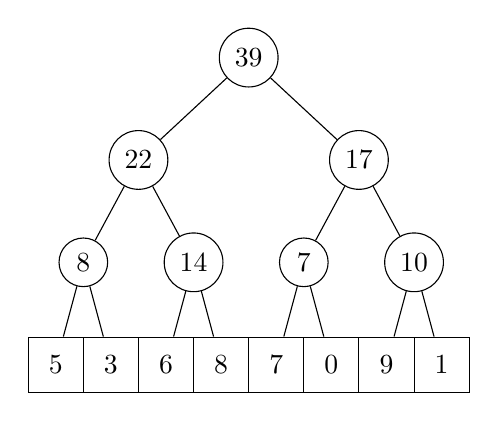
\begin{tikzpicture}[every node/.style={draw},
level 1/.style={sibling distance=28mm,circle,level distance=1.3cm},
level 2/.style={sibling distance=14mm,circle,level distance=1.3cm},
level 3/.style={sibling distance=7mm,rectangle,minimum width=7mm,minimum height=7mm}]
\node[circle]{39}
	child { node{22} 
		child{ node{8} 
			child{ node{5} }
			child{ node{3} }
		}
		child{ node{14} 
			child{ node{6} }
			child{ node{8} }
		}
	}
	child { node{17} 
		child{ node{7} 
			child{ node{7} }
			child{ node{0} }
		}
		child{ node{10}
			child{ node{9} }
			child{ node{1} }
		}
	}
;
\end{tikzpicture}
\end{center}

其中每個節點都對應著一個區間,並且每個區間都會被分為兩個大小差不多的區間,也就是左右兩個子節點代表的區間。在區間求和的問題中,我們會把對應區間的和儲存在節點內,因為線段樹有分塊的性質,所以這個值剛好會等於左右兩個子節點的和。\\

\subsection{我們的節點長怎樣}

為了方便處理區間問題,在一棵線段樹的節點中,我們除了會記錄這個區間的答案(總和)之外,基於實作上方便,還會額外儲存指向兩個子節點的指標,以便操作使用。有的人會在節點裡儲存對應區間的左界與右界,這樣雖然直觀,但是事實上區間的左右界可以在操作過程中計算出,所以如果是競賽程式目的,就不需要浪費空間額外存取左右界。\\

\begin{C++}
struct node(){
    int v;
    node *l, *r;
    node(int v): v(v), l(nullptr), r(nullptr){}
    node(node *l, node* r): l(l), r(r){pull();}
    void pull(){if(l) v = l->v + r->v;}
};
\end{C++}

這裡的 \inline{pull()} 函數類似計算整個分塊的答案,線段樹的每個分塊只有兩個子節點,所以只要對兩個子節點進行處理。這個函數可以根據你所要解決的區間詢問而進行更改,以區間和的詢問為例, \inline{pull()} 函數就是兩子節點的值的和。\\

第$4$行的 constructor 是葉節點的建構元,因為葉節點沒有子節點,所以 \inline{l, r} 兩個指標都指向 \inline{NULL},也因為沒有子節點的緣故,所以必須傳入 \inline{v} 來手動為節點賦值。\\

第$5$行是一般節點的建構元。在樹狀結構中,每個指向節點的指標都可以視為一棵樹,線段樹是一層一層蓋上去的,事實上這個動作能看成在兩棵子樹上新增一個分塊節點,其代表的區間就是兩個子區間合併之後的區間。

\subsection{線段樹的構建}

前面提到過陣列與線段樹的轉換,那麼給定一個陣列,我們要怎麼建構對應的線段樹呢?\\

我們知道一個節點代表的是一段區間,對於一個長度為$n$的序列來説,對應的線段樹的根節點代表的區間就是$[0,n)$,如果這個節點還不是葉節點,無法確定這個節點該有的值,所以要將區間分成兩半,對左右兩半的序列以遞迴的方式分別建立一棵線段樹,直到左右兩節點的值都已經確定,再做一次 \inline{pull()} 操作連結父節點以及兩個子樹並確定父節點的值;如果這個節點已經是葉節點了(也就是區間長度只有1),就代表這個節點的值就是原序列上對應區間(只有一個數)的值,因此只要將對應的值填入即可。\\

\begin{C++}
node *build(int l, int r, int arr[]){
    int mid = l+r >> 1;
    if(l+1 == r) return new node(arr[l]);
    return new node(build(l,mid,arr),build(mid,r,arr));
}
\end{C++}

\hint{因為 \inline{mid} 在這裡面十分常用,所以在實作線段樹時,都會習慣性地加上:\\
\inline{\#define mid l+r>>1}}

宣告一個長度為$n$的線段樹的方式如下:\\

\begin{C++}
node *segTree = build(0, n, arr);
\end{C++}

其中的 \inline{arr} 是一個已經填好值的陣列,建構完的線段樹即可以對這個序列進行區間詢問。

\subsection{查詢區間問題}

我們有了線段樹之後,要怎麼查詢一個區間的總和呢?與分塊一樣,我們可以將詢問區間拆成很多個小區間,這邊有點類似 sparse table 的感覺,但這裡區間必需清楚分割,不允許疊合。比如說要查詢區間$[1,6]$,那就必須查詢以下四個節點。\\

\begin{center}

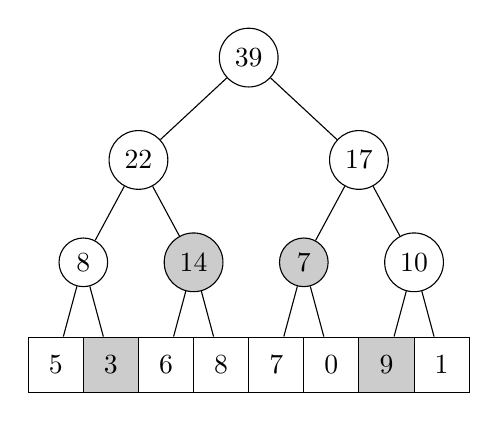
\begin{tikzpicture}[every node/.style={draw},
level 1/.style={sibling distance=28mm,circle,level distance=1.3cm},
level 2/.style={sibling distance=14mm,circle,level distance=1.3cm},
level 3/.style={sibling distance=7mm,rectangle,minimum width=7mm,minimum height=7mm}]
\node[circle]{39}
	child { node{22} 
		child{ node{8} 
			child{ node{5} }
			child{ node[fill=black!20]{3} }
		}
		child{ node[fill=black!20]{14} 
			child{ node{6} }
			child{ node{8} }
		}
	}
	child { node{17} 
		child{ node[fill=black!20]{7} 
			child{ node{7} }
			child{ node{0} }
		}
		child{ node{10}
			child{ node[fill=black!20]{9} }
			child{ node{1} }
		}
	}
;
\end{tikzpicture}
\end{center}

給定一組$l, r$以及一個序列對應的線段樹,我們能在眾多的子節點中選出足夠的節點,使得合併起來的答案就是所求$[l,r]$的解,但總不能全部選擇葉節點吧!一般來說查詢的方法會用到遞迴的概念,從根節點開始根據規則對特定的節點做尋訪,每次遇到一個節點時可以分成三種 case:

\begin{enumerate}
\item 這個節點對應的區間與詢問區間完全互斥:

這個節點的值並不會影響整個詢問的答案,故只要回傳一個無關緊要的答案(也就是合併運算的單位元)就行了。在區間和的問題中,這個值是0;在區間最小值的問題中,這個值是\inline{INF}。

\item 這個節點對應的區間完全包含於詢問區間之內:

這個值將完全影響詢問的答案,因此直接回傳節點的數值即可。

\item 兩個區間互相交錯,只有部分重疊 (即非上述兩種情況):

這個節點無法為答案直接提供任何訊息,只能將區間分成兩半(也就是左右子節點)分別遞迴計算答案,然後再進行一次合併運算決定這個節點的答案。
\end{enumerate}

在實作細節上,我們會實作一個函數,傳入一個節點以及它對應的區間左右界,一開始傳入根節點以及$[0, n)$,再根據情況分成三種 case,不斷遞迴下去。 \\

\begin{C++}
int query(node *a, int l, int r, int ql, int qr){
	  if(r <= ql || qr <= l) return 0; // 互斥
	  if(ql <= l && r <= qr) return a->v; // 完全包含
	  return query(a->l, l, mid, ql, qr) + 
    		   query(a->r, mid, r, ql, qr); // 只有部分重疊
}
\end{C++}

我們多傳了 \inline{ql, qr} 兩個參數,代表詢問區間;每次要詢問時只要呼叫以下函數就完成區間詢問的操作了:\\

\begin{C++}
// 這裡的 l, r 是要詢問的區間,左閉右開。
query(segTree, 0, n, l, r);
\end{C++}

\subsection{修改一個值}

修改是線段樹的靈魂。沒有修改,也不需要線段樹了,前綴就辦的到。那麼當序列的值被更動了之後,我們要怎麼對線段樹修改,才能維持詢問操作的正確答案呢?\\

你會發現當修改序列中的一個值時,只有一些節點會受到影響,如下圖所示:\\

\begin{center}

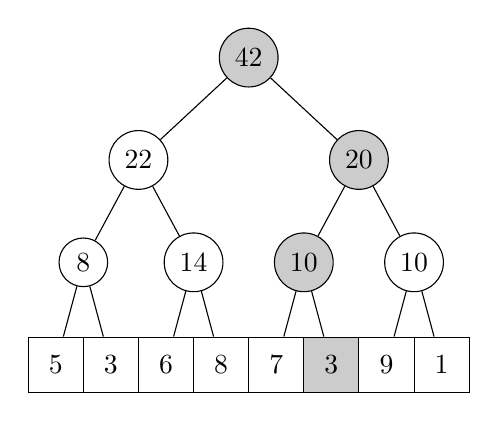
\begin{tikzpicture}[every node/.style={draw},
level 1/.style={sibling distance=28mm,circle,level distance=1.3cm},
level 2/.style={sibling distance=14mm,circle,level distance=1.3cm},
level 3/.style={sibling distance=7mm,rectangle,minimum width=7mm,minimum height=7mm}]
\node[circle,fill=black!20]{42}
	child { node{22} 
		child{ node{8} 
			child{ node{5} }
			child{ node{3} }
		}
		child{ node{14} 
			child{ node{6} }
			child{ node{8} }
		}
	}
	child { node[fill=black!20]{20} 
		child{ node[fill=black!20]{10} 
			child{ node{7} }
			child{ node[fill=black!20]{3} }
		}
		child{ node{10}
			child{ node{9} }
			child{ node{1} }
		}
	}
;
\end{tikzpicture}
\end{center}

更新這些節點的方式十分簡單,一樣從根節點遞迴下去,遇到每個節點就分成三個情況:

\begin{enumerate}
\item 此節點為葉節點:

直接將此節點的值改掉,不需要做任何多餘操作。

\item \inline{pos} 在節點對應區間的左半邊,即 \inline{pos < mid}:

對左子節點遞迴下去,更新完左子樹記得 \inline{pull()} 一下來更新這個節點的值。

\item \inline{pos} 在節點對應區間的右半邊,即 \inline{pos >= mid}:

對右子節點遞迴下去,更新完右子樹記得 \inline{pull()} 一下來更新這個節點的值。
\end{enumerate}

\begin{C++}
void modify(node *a, int l, int r, int pos, int val){
    if(l+1 == r) a->v += val;
    else if(pos < mid) modify(a->l, l, mid, pos, val);
    else modify(a->r, mid, r, pos, val);
    a->pull();
}
\end{C++}

更新序列中的一個值只要簡單的呼叫以下函數就可以達成了:

\begin{C++}
modify(segTree, 0, n, p, v);
\end{C++}

這裏的 \inline{p, v} 就是題目輸入的位置與需要增加的值。

\subsection{線段樹的複雜度}

再來我們來討論線段樹的複雜度。我們先回憶一下我們需要線段樹幹嘛:線段樹提供了區間查詢以及單點修改的操作,這兩個操作可以暴力$\langle O(n), O(1)\rangle$或者前綴$\langle O(1), O(n)\rangle $完成,對於要求比較嚴苛的題目來說,這樣的複雜度還是嫌太慢了,那麼線段樹的複雜度又是如何呢?\\

\subsubsection{操作的代價}

先來看詢問操作:觀察以下的圖示,因為每次查詢的是一個連續區間,所以每層頂多用到左右兩邊各一個節點。如果同一層中有兩個節點需要被尋訪到,則這兩個節點至少有一個必在上一層已經完全涵蓋,可以合併到上一層去。根據這個性質,我們可以知道被尋訪的節點數不會超過\textbf{兩倍樹高},因此詢問的複雜度是$O($樹高$)$。\\

\begin{center}

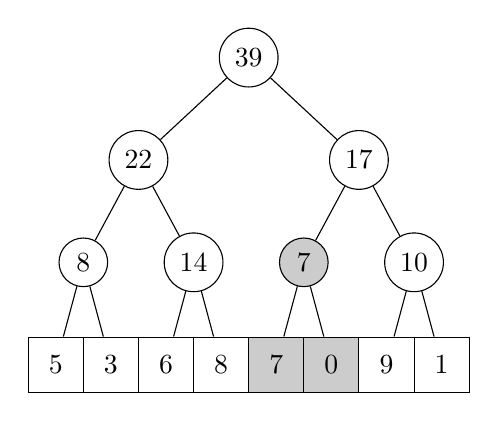
\begin{tikzpicture}[every node/.style={draw},
level 1/.style={sibling distance=28mm,circle,level distance=1.3cm},
level 2/.style={sibling distance=14mm,circle,level distance=1.3cm},
level 3/.style={sibling distance=7mm,rectangle,minimum width=7mm,minimum height=7mm}]
\node[circle]{39}
	child { node{22} 
		child{ node{8} 
			child{ node{5} }
			child{ node{3} }
		}
		child{ node{14} 
			child{ node{6} }
			child{ node{8} }
		}
	}
	child { node{17} 
		child{ node[fill=black!20]{7} 
			child{ node[fill=black!20]{7} }
			child{ node[fill=black!20]{0} }
		}
		child{ node{10}
			child{ node{9} }
			child{ node{1} }
		}
	}
;
\end{tikzpicture}
\end{center}

再來看修改的部分:當尋訪到一個節點時,如果不是葉節點,只會對左子樹或者右子樹遞迴下去,直到碰到需要修改的葉節點為止。因此對於一次修改操作,頂多會尋訪到\textbf{樹高}個節點,因此修改的複雜度也是$O($樹高$)$。

\begin{center}

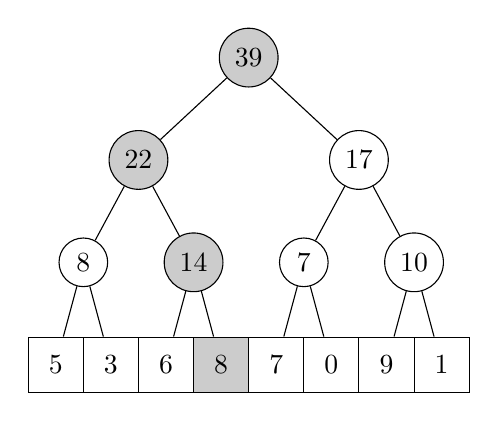
\begin{tikzpicture}[every node/.style={draw},
level 1/.style={sibling distance=28mm,circle,level distance=1.3cm},
level 2/.style={sibling distance=14mm,circle,level distance=1.3cm},
level 3/.style={sibling distance=7mm,rectangle,minimum width=7mm,minimum height=7mm}]
\node[circle,fill=black!20]{39}
	child { node[fill=black!20]{22} 
		child{ node{8} 
			child{ node{5} }
			child{ node{3} }
		}
		child{ node[fill=black!20]{14} 
			child{ node{6} }
			child{ node[fill=black!20]{8} }
		}
	}
	child { node{17} 
		child{ node{7} 
			child{ node{7} }
			child{ node{0} }
		}
		child{ node{10}
			child{ node{9} }
			child{ node{1} }
		}
	}
;
\end{tikzpicture}
\end{center}

\theorem{線段樹的樹高}{
因為線段樹是一棵Complete Binary Tree,也是一棵平衡二元樹,所以一棵有$n$個節點的線段樹的樹高是$O(\log n)$。
}

既然線段樹是一棵平衡二元樹,那麼修改與查詢操作的複雜度也是$O(\log n)$。

\subsubsection{建構的花費}

既然查詢與修改的執行時間都如此迅速,想必是另外多花時間與空間進行預處理的。在這裡我們將討論建構線段樹所需的花費,這邊一定要保持腦袋清晰並銘記在心。\\

首先我們先討論空間複雜度的部分,在這裡先假設序列的長度是二的冪次,如果不是,我們可以在序列後面補0。

我們知道線段樹是多層的分塊,每層是由下面的兩個節點組成。因此對於線段樹的每一層,節點數都會是下面一層的一半。將每層的所有節點數加起來,整棵樹的節點數就是$n+\frac{n}{2}+\frac{n}{4}+...+1=2n$。

\hint{\textbf{重要!} 線段樹的空間複雜度是$O(n)$,不是$O(n\log n)$。}

再來是時間複雜度。這部分比較簡單,因為建構一個節點只是單純的呼叫一次建構元以及 \inline{pull()} 函數,因此時間複雜度與空間複雜度相同,皆是$O(n)$。

\theorem{線段樹的複雜度}{
建構一個序列長度為$n$的線段樹需要$O(n)$的時間以及$O(n)$的空間。\\
對於一個序列長度為$n$的線段樹,查詢以及修改的時間複雜度皆為$O(\log n)$。
}

\subsection{一定要指標嗎}

其實線段樹不一定要用上述的指標型來實作,因為線段樹是一棵Complete Binary Tree,所以其實陣列是一個不錯的選擇,陣列型線段樹的優點將會在接下來的內容提到。

\subsubsection{快速改造--陣列線段樹}

指標型的線段樹要改成陣列其實十分的簡單,通常一個熟悉線段樹實作的人能在十分鐘內改造完畢。\\

在之前的章節中,我們有提到過二元樹的陣列表示法--利用編號$2n$與$2n+1$的節點為編號$n$的節點的左右子樹,其中編號$1$是樹根。以下是節點與編號的對應:\\

如果 \inline{a} $\rightarrow$ $i$,則
\begin{itemize}
\item \inline{a->l} $\rightarrow$ $2i$
\item \inline{a->r} $\rightarrow$ $2i+1$
\end{itemize}

我們用個陣列來儲存節點的值,也就是說

\begin{itemize}
\item \inline{a->v} $\rightarrow$ \inline{segTree[i]}
\end{itemize}

最後注意一下實作細節,將 \inline{idx} (即節點編號)一起傳入函數,方便做陣列處理即可。\\

以下是陣列線段樹的程式碼:\\

\begin{C++}
int segTree[4*MAX_N];

void pull(int idx){
    segTree[idx] = segTree[2*idx] + segTree[2*idx+1];
}

void build(int l, int r, int arr[], int idx = 1){
    if(l+1 == r) segTree[idx] = arr[l];
    else build(l, mid, arr, 2*idx), 
        build(mid, r, arr, 2*idx+1), pull(idx);
}

int query(int l, int r, int ql, int qr, int idx = 1){
    if(r <= ql || qr <= l) return 0;
    if(ql <= l && r <= qr) return segTree[idx];
    return query(l, mid, ql, qr, 2*idx) + 
           query(mid, r, ql, qr, 2*idx+1);
}

void modify(int l, int r, int pos, int val, int idx=1){
    if(l+1 == r) segTree[idx] += val;
    else if(pos < mid) modify(l, mid, pos, val, 2*idx);
    else modify(mid, r, pos, val, 2*idx+1);
    pull(idx);
}
\end{C++}

注意這裡的陣列要開四倍,不然在修改或者查詢的操作中可能會超出陣列外面,造成SF。

\hint{線段樹要開四倍,不是兩倍,更不是$\log n$倍。}

從這邊可以看出陣列型與指標型線段樹的微小差別:\\
\url{https://drive.google.com/file/d/1l6fLCyxqCZS4TgBStCUoUMArfcg5Qo5f/view?usp=sharing}

\subsubsection{陣列線段樹有什麼好處}

首先,最直接的就是記憶體用量。一個指標要占 8bytes ,一個節點就至少要 20bytes,而陣列只要區區四個位元組。有些題目故意卡記憶體就會卡到指標。再者,指標的存取速度比較慢,遇到卡常數的題目就會TLE。有時候線段樹的初始值要全部都是0,這時候指標的 \inline{build()} 函數就會執行過慢導致逾時;而陣列一宣告就可以自動填上0,甚至不需要呼叫 \inline{build()} 函數。

另外還有一種偽指標的方法,也就是在一開始開好一個拿來當記憶體池的陣列,並且以陣列的索引值代替指標,如此能夠省下部分的空間複雜度,實作上只需要把指標型的程式碼中\inline{new}的部分改為回傳一個空的陣列索引即可。

\section{BIT 樹狀數組}
	BIT,是 Binary Indexed Tree 的簡稱,最早由 Peter Fenwick 所發明,因此又稱作 Fenwick Tree,中文譯作樹狀數組,是一個拿來處理動態前綴和的資料結構,以下我們將直接簡稱 BIT。\\
	讓我們先看看題目~
\problem{經典題 - 動態前綴和 (No judge)}{
給定一個序列 $a_1, a_2, \dots , a_n$,之後有 $q$ 筆操作,操作有以下兩種:查詢前 $i$ 項的和、修改 $a_i$ 的值。 $n,q\leq 10^5$
}
\par 對於這樣一個看起來很簡單的問題,大家可能會想到兩種解法:
\begin{itemize}
\item 每次詢問時便計算一次 $a_1 + a_2 + \dots + a_i$,修改時直接修改該項的值即可。詢問複雜度 $O(N)$、修改複雜度 $O(1)$
\item 用一個陣列 pre 來維護前 $i$ 項的和,詢問時直接輸出答案,修改時則需要改變 pre[$i$] ~ pre[$n$] 的值。詢問複雜度 $O(1)$、修改複雜度 $O(N)$
\end{itemize}

\par 這兩種方法分別將複雜度花在了詢問或修改上,但總複雜度一樣都是 $O(NQ)$,這時候便出現了一種想法,有沒有可能讓詢問及修改的複雜度盡可能平均,而降低總複雜度呢?\\

\par 如果有認真看前面講義的人,可能就會想到可以利用線段樹來解決這個問題,而在刻線段樹的同時,大家會發現對於每個 node,左子節點的值加上右子節點的值其實就是這個 node 自己本身的值。我們便利用這樣的性質對這棵線段樹進行一點優化,試著將右子節點全部刪掉,然後用左子節點和節點本身來表示右子節點的值,這就是 BIT 最重要的精神!\\

\par 那麼,這樣一顆奇形怪狀的樹到底該怎麼維護呢?經過一番整理與歸納後我們會發現,在這棵樹上的每個節點的範圍 $[l, r]$ 中,每個 $r$ 會對應到唯一的 $l$,這表示我們只要用一個陣列來記錄這些節點的值就行了,我們且將這個陣列稱作 BIT。\\

\par 接著我們要討論到底該如何完成 BIT 陣列,由前面討論出我們所要記錄的節點,可以發現這些節點所記錄的區間其實就相當於 $i$ 以二進位表示後最低位的 1 的位置(之後稱之為 lowbit$(i)$),例如 $26_{10} = 11010_{2}$,BIT[26] $= [26-$lowbit$(26)+1, 26] = [25, 26]$,而預處理這樣的陣列也有個簡單的作法,我們維護當前的前綴pre[$i$],那麼 BIT[$i$] 就會等於 pre[$i$] - pre[$i-$lowbit$(i)$],便能以 $O(N)$ 預處理建出 BIT 陣列了。\\

\par 完成了 BIT 陣列的建置後,便可以開始進行操作了,我們先以詢問的角度來看,對於每次的詢問 $[1, k]$,將詢問分為 $[1, k-$lowbit$(k)]$ 與 $[k-$lowbit$(k)+1, k]$ 兩部分,根據上段所述,我們能以 $O(1)$ 求得後項的答案,之後再對前項遞迴下去,最多只需 $\log{N}$ 次,便能得到 $[1, k]$ 的值了。\\

\par 接下來是修改的部分,當我們修改 $a_i$ 的值時,考慮到被影響的內容是 BIT[$i$]、BIT[$i+$lowbit$(i)]\cdots$(有點通靈,請大家認真思考一下),於是我們便遞迴下去,僅需 $O(\log_2{N})$ 即可完次成對 BIT 陣列的修改。\\

\par 順帶一提,計算 lowbit$(k)$ 的方式也不難, lowbit$(k) = k \& ($~$k + 1 )$ ($\&$ 是 bitwise-and、~ 是 bitwise-not),而利用目前大部分的處理器架構中,負數其實就是2補數(反轉再加一)的特性,又可以直接寫作 $k \& -k$。\\

\begin{C++}
int a[N+1], pre[N+1], bit[N+1];
inline int lowbit(int n) { return n&-n; }
void build() {
  for (int i = 1; i <= N; i++) 
    bit[i] = pre[i] - pre[i-lowbit(i)];
}
int sum(int n) {
	int ret = 0;
	for(;n;n-=lowbit(n)) ret += bit[n];
	return ret;
	//類似將n以二進位分解
}
void add(int n, int v) {
	for(;n<=N;n+=lowbit(n)) bit[n] += v;
	//想像更新編號為n的節點的所有父節點
}
\end{C++}

\par 初始化、詢問、修改三個函式各自的程式碼都不超過 $3$ 行,這應該是各位除了 STL 外會接觸到最親民的資料結構了,因此一定要好好把握。

\par 最後來統整一下複雜度吧!按照前面所講的作法,預處理 $O(N)$、每次查詢或修改 $O(\log{N})$,總複雜度為 $O(Q\log{N})$,複雜度不輸線段樹,coding 複雜度又低,無怪它這麼受人歡迎呢!

\subsection{值域BIT}
話不多說,請大家看看例題吧
\problem{經典題 - 逆序數對 (TIOJ 1080)}{
給定一個序列 $a_1, a_2, \dots , a_n$,詢問此序列中有多少對 $(i, j)$ ,使得 $i < j$ 且 $a_i > a_j$。 $n\leq 10^5$
}
\par 看到這個題目很容易發現,我們只要統計每個 $a_i$ 前面比它大的數字並加總,便能得到答案了,現在的問題只剩下,要怎麼快速知道每個 $a_i$ 前面有多少個比它大的數呢?這時候我們的 BIT 就派上用場了,首先定義 ans 表示答案,然後我們讓 BIT[$a_i$] 表示目前有多少個 $a_i$,接著我們從 $a_0$ 開始,每次讓 ans 加上 $(i - [1, a_i])$ 表示當前比 $a_i$ 大的數的數量,接著將 $a_i$ 加入 BIT 陣列中,完成後便能得到我們的答案,而這就是所謂值域 BIT 的概念。
\begin{C++}
int num[N+1], bit[N+1], ans;
inline int lowbit(int n) {return n & -n;}
int sum(int n) {
  return n ? bit[n] + sum(n-lowbit(n)) : 0;
}
void add(int n, int v) {
  bit[n] += v;
  if (n <= N) add(n+lowbit(n),v);
}
int main() {
  for (int i = 0; i < N; i++) {
    ans += i-sum[num[i]];
    add(num[i], 1);
  } 
  return 0;
}
\end{C++}
\subsection{區間加值\&單點查詢}
接下來開始是一些進化版的 BIT
\problem{區間加值\& 單點查詢 (No judge)}{
給定一個序列 $a_1, a_2, \dots , a_n$,之後有 $q$ 筆操作,操作有以下兩種:查詢第 $i$ 項的值、使區間 $[l, r]$ 同時 $+k$。$n,q\leq 10^5$
}
\par 這問題感覺與普通的 BIT 有種似曾相識的感覺(?,差別只在於這次我們是一次修改一個區間,而查詢也縮成了一次只查詢一個點,對於這樣的問題,我們可以想想該如何變化我們的 BIT 。首先,一次必須修改一個區間,我們勢必不能對這個區間內的值一個一個修改,因此,我們會需要用到一個與前綴恰恰相反的方法-差分,我們先建立原數列的差分陣列 d,而第 $i$ 項的值就是 $[1, i]$ 的前綴和,接著來看看修改的部分,當我們將區間 $[l, r]$ 同時 $+k$,也就表示我們讓 d[$l$] 的值 $+k$、d[$r+1$] 的值 $-k$,如此一來便能成功用 BIT 達成區間加值\& 單點查詢了。
	\subsection{區間加值\&區間查詢}
	再更進階一點...
\problem{區間加值動態前綴和 (No judge)}{
給定一個序列 $a_1, a_2, \dots , a_n$,之後有 $q$ 筆操作,操作有以下兩種:查詢前 $i$ 項的和、使區間 $[l, r]$ 同時 $+k$。$n,q\leq 10^5$
}
\par 情況似乎又變得更複雜了...,這次似乎無法單靠將原本的陣列轉成差分便求得答案,這時候我們決定先將詢問轉化看看:
$$\sum_{i=1}^{n} a_i = \sum_{i=1}^{n}\sum_{j=1}^{i} d[j]$$
考慮每個$d[j]$被加到的次數
$$\sum_{i=1}^{n}\sum_{j=1}^{i} d[j] = \sum_{i=1}^{n} (n-i+1) \cdot d[i] = (n+1) \cdot \sum_{i=1}^{n} d[i] - \sum_{i=1}^{n} i \cdot d[i]$$
因此我們可以利用兩個 BIT 來做到區間加值 \& 查詢!,一個 BIT 維護 d[$i$],另一個維護 $i \cdot$ d[$i$],然後再用上述的方法合併,修改的部分如前一小節所述。
	\subsection{更高維的版本}
	BIT 動態前綴和推廣成高維版本的方式,就是使 BIT 的每一項都成為一個 BIT ,這樣便是一個二維 BIT 了,至於複雜度的話,每多增加一維,便會變為 $\log{N}$ 倍,因此複雜度為 $O(\log{N}^DQ)$,但倘若是要查詢任意區間的話,就必須要使用排容原理,複雜度 $O(2^D\log{N}^DQ)$ 。
	
\section{Sparse Table}
sparse table 主要是處理 RMQ (區間最小值)的問題,為倍增法的一種實現。

考慮到暴力建表需要$O(N^2)$的複雜度,我們發現以下的性質:
\begin{center}
$min(a,b)=min(a,b,b)$\\
\end{center}
也就是說,一段區間詢問的拆解是可以拆成有交集的區間(因為相同數字重複取$min$並不會影響答案)。如此一來,我們只要想辦法用某些長度的聯集湊出任意區間,就能加快詢問速度了。但我們該用哪些長度湊出這些區間呢?想起來我們的前言了嗎?沒錯,實際上用長度為$2$的冪次的區間來處理會是最有效的。那對於某段區間$[l,r)$,我們該如何拆解呢?我們只要找到滿足下列式子的$d$即可:
\begin{center}
$\frac{r-l}{2} \leq d=2^k\leq r-l$
\end{center}
不難發現$k=[\log _2 (r-l)]$,$d=2^k =2^[\log _2 (r-l)]$。因此$min([l,r))=min([l,l+d),[r-d,r))$。於是我們建立一個 st 表格,其中st$[i][j]$代表編號在$[j,j+2^i)$範圍內的最小值。這樣一來只要將詢問轉換一下就可以$O(1)$查詢了。
\subsection{預處理}
建表時不難發現以下式子:
$$\begin{cases}
$st$[i][0]=a[i]\\
$st$[i][j]=min($st$[i-1][j],$st$[i-1][j+2^{i-1}])
\end{cases}$$
表格總共$\log _2 N$行$N$列,可以$O(N\log N)$ dp建完。
\subsection{查詢}
查詢時根據上述原理將輸入範圍$[l,r)$轉換為$[l,l+2^{[\log _2 (r-l)]})$和$[r-2^{[\log _2 (r-l)]},r)$兩段,於是$[l,r)$的答案就會是$min($st$[[\log _2 (r-l)]][l],$st$[[\log _2 (r-l)]][r-2^{[\log _2 (r-l)]}])$,達成$O(1)$查詢。\\\\
以下是程式碼:
\begin{C++}
int a[maxn],st[(int)log2(maxn)+1][maxn];
void build(int n){
    for(int i=0;i<n;i++) st[0][i]=a[i];
    for(int l=1,i=1;i<=(int)log2(n);i++,l<<=1)
        for(int j=0;j+l<n;j++)
            st[i][j]=min(st[i-1][j],st[i-1][j+l]);
}
int query(int l,int r){
	return min(st[(int)log2(r-l)][l],st[(int)log2(r-l)][r-1<<((int)log2(r-l))]);
}
\end{C++}
\subsection{小小的推廣}
上述sparse table的min運算可替換為「具交換律、結合律且滿足$f(x,x)=x$」的任意二元運算$f$。\\
\problem{胖胖殺蚯事件(TIOJ1603)}{給定$n$棟大樓高度$h[i]$和$m$筆詢問$[l,r]$,輸出每筆詢問區間的最大值$-$最小值。}

\end{document}
